\RequirePackage{luatex85}
\documentclass{standalone}

\usepackage{fontspec, unicode-math}
\setsansfont[Scale=MatchLowercase]{TeX Gyre Heros}
\setmathfont{TeX Gyre Termes Math}

\usepackage{tikz}
\usetikzlibrary{arrows.meta}

\tikzset{
  every picture/.style={font={\sffamily\normalsize}, >=stealth},
  every pin edge/.style={black}}

\begin{document}

  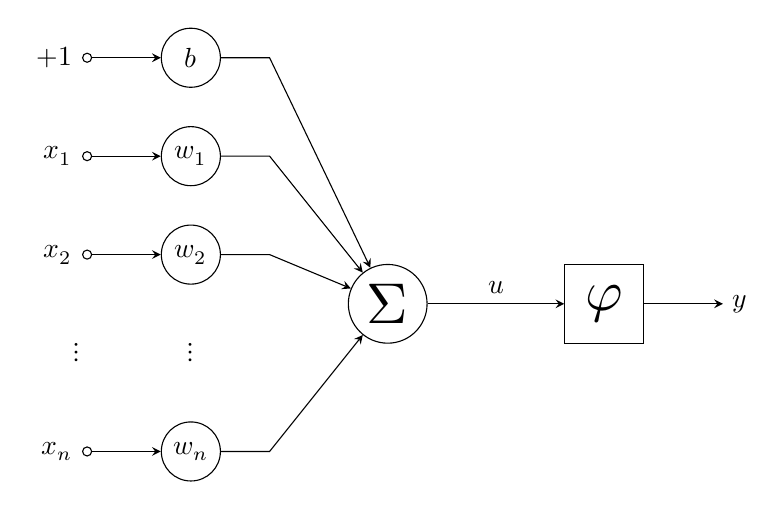
\begin{tikzpicture}
    \tikzstyle{perceptron}=[draw, font=\huge, minimum size=1cm, inner sep=0pt]

    \begin{scope}[every circle node/.style={%
      draw, minimum size=0.75cm, inner sep=0pt}, pin edge={<-{Circle[open]}}, pin distance=1cm]

      \node[circle] (E) at (0, 5)    [pin={left:$+1$}] {$b$};
      \node[circle] (A) at (0, 3.75) [pin={left:$x_{1}$}] {$w_{1}$};
      \node[circle] (B) at (0, 2.5)  [pin={left:$x_{2}$}] {$w_{2}$};
      \node[circle] (D) at (0, 0)    [pin={left:$x_{n}$}] {$w_{n}$};
    \end{scope}

    \node[circle] (C) at (0, 1.25) [pin={[pin edge=white, pin distance=1cm]left:$\vdots$}] {$\vdots$};

    \begin{scope}
      \draw (2.50, 1.875) node[circle, perceptron] (S) {$\Sigma$};
      \draw (5.25, 1.875) node[rectangle, perceptron, pin={[pin edge={->}, pin distance=1cm]right:$y$}]
        (F) {$\varphi$};
    \end{scope}

    \begin{scope}
      \draw[->] (E) to (1, 5)    to (S);
      \draw[->] (A) to (1, 3.75) to (S);
      \draw[->] (B) to (1, 2.5)  to (S);
      \draw[->] (D) to (1, 0)    to (S);
    \end{scope}

    \draw[->] (S) to [edge label=$u$] (F);
  \end{tikzpicture}

\end{document}
